\documentclass[11pt, a4paper,twocolumn]{jarticle}
\usepackage[dvipdfmx]{graphicx}
\usepackage{listings,jlisting}

\begin{document}
%=============================================================
\section{Measure of the resistivity($2^{nd} day$)}

\subsection{Purpose}
金属の電流電圧特性を測定する.
\subsection{Procedure}
4端子測定法により以下に示す試料の抵抗を求める.
測定した抵抗値から試料の長さ,直径を考慮してそれぞれの試料の抵抗率を求める.
また今回の測定は全てl = 1cmの幅で行った.
\begin{itemize}
    \item A copper wire
    \item A NiCr wire
    \item A tungsten wire
    \item A lead of automatic pencil(H,2B)
    \item A Ni wire
    \item An Ag wire
    \item An unknown sample
\end{itemize}
\subsection{Result}
測定の結果電流電圧の関係をプロットすると以下のようなグラフが得られた.

\begin{figure}[htbp]
 \begin{center}
  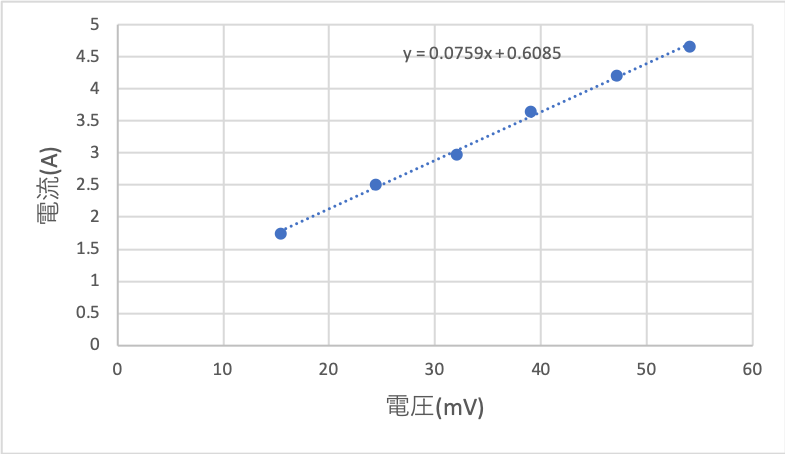
\includegraphics[width=0.8\linewidth]{fig15.png}
 \end{center}
 \caption{Cu}
 \label{fig:15}
\end{figure}

\begin{figure}[htbp]
 \begin{center}
  
\includegraphics[width=0.8\linewidth]{fig16.png}
 \end{center}
 \caption{NiCr}
 \label{fig:16}
\end{figure}

\begin{figure}[htbp]
 \begin{center}
  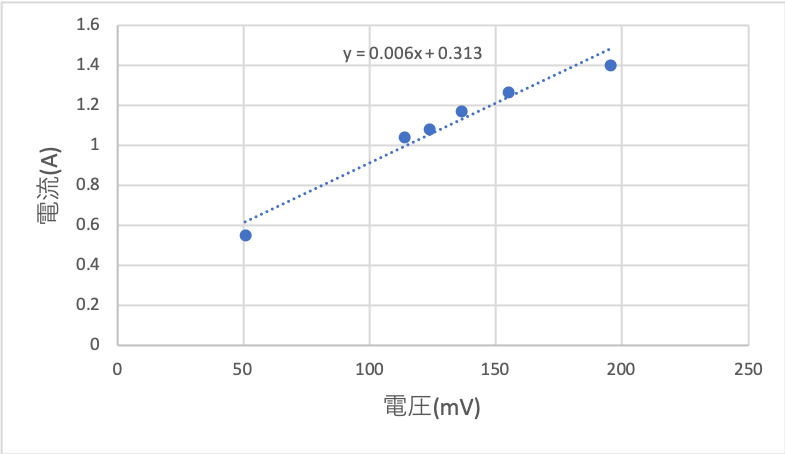
\includegraphics[width=0.8\linewidth]{fig17.png}
 \end{center}
 \caption{W}
 \label{fig:17}
\end{figure}

\begin{figure}[htbp]
 \begin{center}
  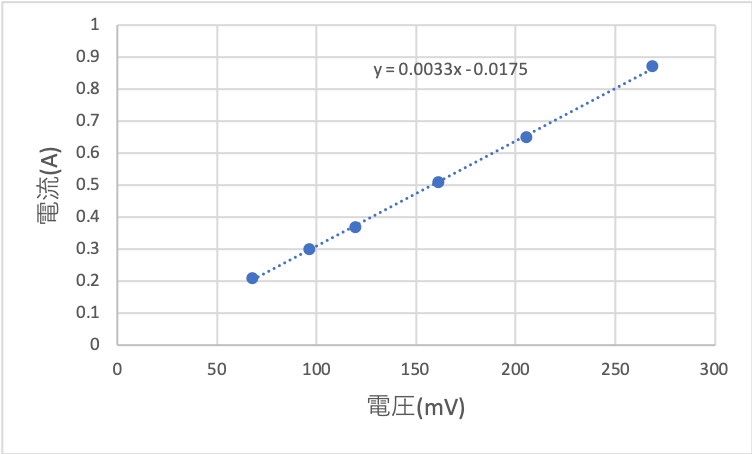
\includegraphics[width=0.8\linewidth]{fig18.png}
 \end{center}
 \caption{シャープペンシルの芯H}
 \label{fig:18}
\end{figure}

\begin{figure}[htbp]
 \begin{center}
  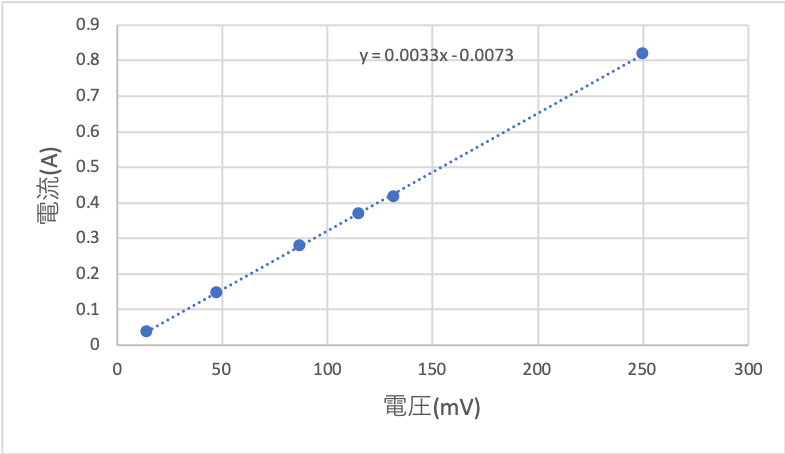
\includegraphics[width=0.8\linewidth]{fig19.png}
 \end{center}
 \caption{シャープペンシルの芯2B}
 \label{fig:19}
\end{figure}

\begin{figure}[htbp]
 \begin{center}
  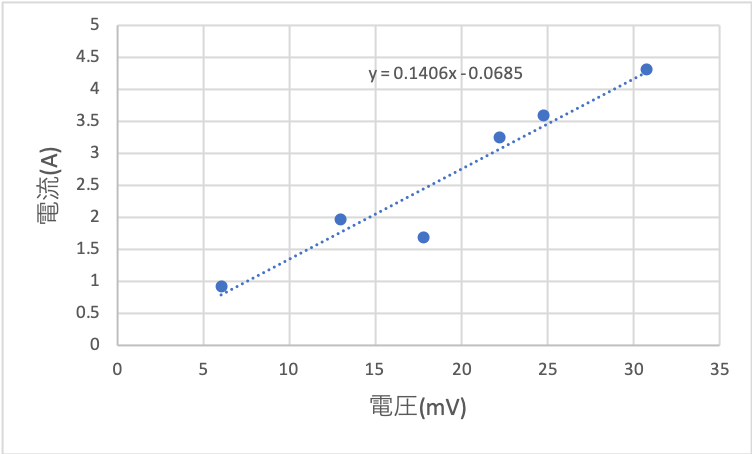
\includegraphics[width=0.8\linewidth]{fig20.png}
 \end{center}
 \caption{Ni}
 \label{fig:20}
\end{figure}

\begin{figure}[htbp]
 \begin{center}
  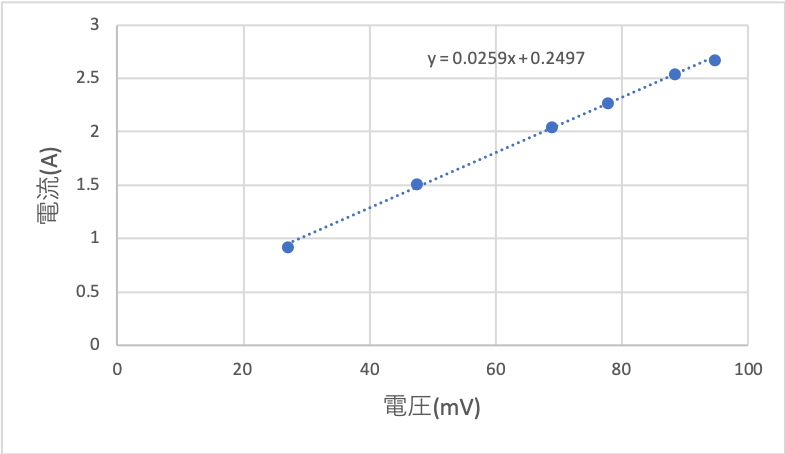
\includegraphics[width=0.8\linewidth]{fig21.png}
 \end{center}
 \caption{Ag}
 \label{fig:21}
\end{figure}

\begin{figure}[htbp]
 \begin{center}
  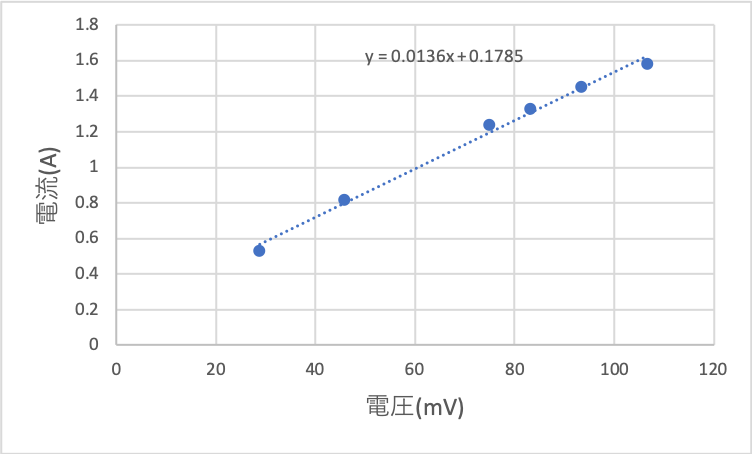
\includegraphics[width=0.8\linewidth]{fig22.png}
 \end{center}
 \caption{不明試料}
 \label{fig:22}
\end{figure}


以上の結果よりグラフの傾きを最小二乗法によって求めそれぞれの抵抗値,抵抗率を求めたところ以下の表のようになった.

\begin{table}[htb]
  \begin{center}
      \caption{抵抗値,抵抗率}
        \begin{tabular}{|c|c|c|} \hline
             試料(直径mm) & 抵抗値($\Omega$) & 2端子($\mu\Omega$cm) \\ \hline
             Cu(0.18) & 0.0132 & 3.35 \\
             NiCr(0.17) & 0.556 & 126 \\
             W(0.09) & 0.1667 & 10.6 \\
             \begin{tabular}{c}
                シャープペンシル \\ の芯H(0.5)
             \end{tabular}
             & 0.3030 & 594 \\
            \begin{tabular}{c}
                シャープペンシル \\ の芯2B(0.5)
            \end{tabular}
             & 0.3030 & 594 \\
             Ni(0.9) & 0.0711 & 45.2 \\
             Ag(0.07) & 0.0386 & 1.49 \\
             不明(0.195) & 0.0735 & 22.0 \\ \hline
        \end{tabular}
  \end{center}
\end{table}

\subsection{Discussion}
どの試料金属においても温度が上昇するにつれて低効率が高くなった現象について考察する.
まず金属はエネルギーバンド図において伝導体に電子を常に持っておりこれは自由電子として電流を運ぶ役割を果たしている.
ここで温度が上昇した場合は格子が熱でより激しく振動することになると予想される.
したがって電子の通り道を格子が塞ぐ確率が高まり結果として単位時間に電子が衝突する回数が多くなり抵抗率が温度の上昇とともに上昇していくと考えられる.
またこの現象から,電子の量が多くなることにより格子に衝突する電子の量が多くなることが予測される.
これはオームの法則の説明であると考えられる.

また測定結果より未知試料だと思われる物質はストロンチウムだと考えられる.
しかし他の金属試料において抵抗率のオーダーはあっているもののその値は理科年表の値から多少ずれており測定において接触抵抗などのノイズが入ったことが考えられる.

またシャープペンシルの芯は濃さに寄らず同じ値を示したことから濃さに寄らずに同じ構造をしていることが予想される.またシャープペンシルの芯はグラフェンであり結合に余分な価電子によって電流を通すが自由電子の数は金属に比べ少ないことが結果から考えられる.
%=============================================================
\newpage
\end{document}
